\documentclass[11pt,a4 paper]{article}
\usepackage{subfiles}

\usepackage{amsmath, amsthm}
\usepackage[english]{babel}
\usepackage[T1]{fontenc}
\usepackage[utf8]{inputenc}
\usepackage[margin=2cm]{geometry}
\usepackage{graphicx}
%\usepackage{subfig}
\usepackage{caption}
\usepackage{subcaption}
\usepackage{siunitx}
\captionsetup{tableposition=top,font=small,width=0.8\textwidth}
\usepackage{booktabs}
\usepackage[table]{xcolor}
\usepackage[arrowdel]{physics}
\usepackage{mathtools}
\usepackage{tablefootnote}
\usepackage{amssymb}
\usepackage{enumitem}
\usepackage{mathcomp}
\usepackage{multicol}
\setlist[description]{font={\scshape}} %style=unboxed,style=nextline
\usepackage{wrapfig}
\usepackage{float}
\usepackage{import}
\usepackage{floatflt}
\usepackage{url}
\usepackage{commath}
\usepackage{bm}
\usepackage[version=4]{mhchem}
\usepackage{nicefrac}
\usepackage{ifthen}
\usepackage{comment}
\usepackage[colorinlistoftodos,textsize=tiny]{todonotes}
\usepackage{hyperref}

\renewcommand*{\thefootnote}{\fnsymbol{footnote}}
\sisetup{exponent-product = \cdot}
\newcommand{\tc}{\,\mbox{tc}\,}
\newcommand{\Epsilon}{\mathcal{E}}
\newcommand{\half}{\frac{1}{2}}
\newcommand{\overbar}[1]{\mkern 1.5mu\overline{\mkern-1.5mu#1\mkern-1.5mu}\mkern 1.5mu}
\let\oldfrac\frac
\renewcommand{\frac}[3][d]{\ifthenelse{\equal{#1}{d}}{\oldfrac{#2}{#3}}{\nicefrac{#2}{#3}}}

\title{VESPA\\Vaso per Esperimenti Su Plasmi ed Altro}
\author{Andrea Grossutti, mat. 1237344\\Alessandro Lovo, mat. 1236048\\Leonardo Zampieri, mat. 1237351}
\date{\today}

\begin{document}

\maketitle

\section{Aims}
Study the \emph{Vespa} experimental apparatus, and in particular:
\begin{itemize}[noitemsep]
    \item Model the vacuum system behavior, finding the characteristic parameters;
    \item Obtain the current-voltage and the current-temperature characteristics curves of the filament;
    \item Draw the voltage-current characteristics curves of the gas discharge, enhancing their behavior as varying pressure;
    \item Find the Paschen curve, both in DC and RF condition;
    \item Measurement of plasma parameters through a Langmuir probe, both in stationary conditions and via ionic-sonic wave propagation.
\end{itemize}


\section{Vacuum system}
The vacuum inside the VESPA vessel (a cylindrical  vessel, with a length of $\sim80\si{\centi\metre}$ and a radius of $\sim20\si{\centi\metre}$: $V\sim0.1\si{\metre^3}$) is obtained and kept thanks to a rotary pump and a turbomolecular pump. The vessel is not perfectly isolated and some small leaks affect the vacuum keeping. To study this phenomena, the vessel has been taken to a low pressure ($\sim 6 \cdot 10^{-5} \si{\milli\bar}$) and all the valves around have been closed. Isolating the chamber from the pumping system one can measure (thanks to a ionization pressure gauge) the pressure in the vessel as function of time. Effects as leaks and degasing contribute to an inflow in the chamber $F_0(p)$ that in principle could depend on the pressure. Assuming instead $F_0$ constant, its value can be estimated through a linear fit on the data: $P = a + b \cdot t$, $F_0 = V \cdot b$.

Considering the reaction time, the slowness of the ionization gauge in stabilizing and the pressure oscillations, the errors are estimated as $5\%$ on the pressure and $0.5\si{\second}$ error on the time.

\begin{figure}[H]
  \centering
  \resizebox{0.5\textwidth}{!}{\import{img/vacuum/}{increase_all_fit.tex}} \hspace{-0.05\textwidth}
  \resizebox{0.5\textwidth}{!}{\import{img/vacuum/}{increase_all_residuals.tex}}
  \caption{Presure increasing in the chamber}
  \label{fig:increase_all}
\end{figure}

As can be seen from fig \ref{fig:increase_all} there is an evident trend in the residuals, proving that $F_0$ cannot be assumed constant throughout all the explored range of pressures. A possible way to correct this is to consider a low pressure regime and a high pressure one: the limit has been put where the trend in the residuals inverts, i.e. around 200\si{\nano\pascal}.
\begin{figure}[H]
  \centering
  \resizebox{0.5\textwidth}{!}{\import{img/vacuum/}{increase_lowP_fit.tex}} \hspace{-0.05\textwidth}
  \resizebox{0.5\textwidth}{!}{\import{img/vacuum/}{increase_lowP_residuals.tex}}
  \caption{Low pressure regime}
  \label{fig:increase_lowP}
\end{figure}
\begin{figure}[H]
  \centering
  \resizebox{0.5\textwidth}{!}{\import{img/vacuum/}{increase_highP_fit.tex}} \hspace{-0.05\textwidth}
  \resizebox{0.5\textwidth}{!}{\import{img/vacuum/}{increase_highP_residuals.tex}}
  \caption{High pressure regime}
  \label{fig:increase_highP}
\end{figure}
% \todo[inline]{Secondo me è un po' un casino, un po' tutto stretto. Proporrei invece al posto delle figure \ref{fig:increase_highP} e \ref{fig:increase_lowP} la figura seguente:}

% \begin{figure}[H]
%   \centering
%   \resizebox{0.8\textwidth}{!}{\import{img/vacuum/}{combined.tex}}
%   \caption{Fits in the two regimes.}
%   \label{fig:increase_combined}
% \end{figure}

% \todo[inline]{REPLY: secondo me no: i residui ci stanno}
Splitting the high pressure regime and the low pressure one two different estimation of the inflow can be computed:
\begin{gather*}
  F_0^\text{low} = (6.4 \pm 0.4) \cdot 10^{-6} \si{\pascal}\, \si{\metre^3}/\si{\second}, \quad
  F_0^\text{high} = (4.5 \pm 0.4) \cdot 10^{-6} \si{\pascal}\, \si{\metre^3}/\si{\second}
\end{gather*}
where a 5\% error on the volume is assumed.

Subsequently, the valve has been opened connecting the chamber to the pumping system. An exponential lowering of the pressure is expected: $P(t) = (P_i - P_0)e^{-\frac[f]{t}{\tau}} + P_0$, where $P_i$ is the starting pressure and $P_0$ the asymptotic one.

\begin{figure}[H]
  \centering
  \resizebox{0.5\textwidth}{!}{\import{img/vacuum/}{decrease_all_fit.tex}} \hspace{-0.05\textwidth}
  \resizebox{0.5\textwidth}{!}{\import{img/vacuum/}{decrease_all_residuals.tex}}
  \caption{Pressure lowering in the chamber}
  \label{fig:decrease_all}
\end{figure}

As can be seen from fig \ref{fig:decrease_all}, similarly as what seen before, the result are not acceptable and as before two regimes can be distinguished. For coherence and for a better comparison, the same limit previously chosen has been used.

\begin{figure}[H]
  \centering
  \resizebox{0.5\textwidth}{!}{\import{img/vacuum/}{decrease_lowP_fit.tex}} \hspace{-0.05\textwidth}
  \resizebox{0.5\textwidth}{!}{\import{img/vacuum/}{decrease_lowP_residuals.tex}}
  \caption{Low pressure regime}
  \label{fig:decrease_lowP}
\end{figure}

\begin{figure}[H]
  \centering
  \resizebox{0.5\textwidth}{!}{\import{img/vacuum/}{decrease_highP_fit.tex}} \hspace{-0.05\textwidth}
  \resizebox{0.5\textwidth}{!}{\import{img/vacuum/}{decrease_highP_residuals.tex}}
  \caption{High pressure regime}
  \label{fig:decrease_highP}
\end{figure}

% \todo[inline]{Facendo un grafico in scala logaritmica, sembra invece che ci siano tre regimi! Vedere figura seguente}

% \begin{figure}[H]
%   \centering
%   \resizebox{0.8\textwidth}{!}{\import{img/vacuum/}{combined_emptying.tex}}
%   \caption{Fits in different regimes.}
%   \label{fig:combined_emptying}
% \end{figure}

% \todo[inline]{REPLY: secondo me no: 1) Il regime intermedio non sembra un gran che: c'\`e forte andamento nei residui. 2) tenendo solo due regimi si riesce a fare meglio il confronto pi\`u avanti}


Performing two separate exponential fits, they result in a meaningful result (even if a small trend in residual is still visible). From the values of $\tau$ and $P_0$ the effective pumping speed $S_e$, the inflow $F_0$ and, given the nominal value of the pumping speed $S = 33 \si{\litre/\second}$, the conductance of the chamber-pump connection $C$ can be estimated.

\begin{table}[H]
  \centering
  \begin{tabular}{cccccc}
    \toprule
    Regime & $S_e = \frac[f]{V}{\tau}\,[\si{\litre\per\second}]$ & $F_0 = P_0 \cdot S_e\,[\si{\pascal\,\metre^3\per\second}]$ & $C = (S_e^{-1} - S^{-1})^{-1}\,[\si{\litre\per\second}]$ \\
    \midrule
    Low pressure & $0.51 \pm 0.04$ & $(2.2 \pm 0.2)\cdot 10^{-6}$ & $0.52 \pm 0.05$ \\
    High pressure & $4.0 \pm 0.6$ & $(2 \pm 1)\cdot 10^{-5}$ & $4.6 \pm 0.7$ \\
    \bottomrule
  \end{tabular}
  \caption{Vacuum parameters}
  \label{tab:vacuum}
\end{table}

In the low pressure regime the two estimates of $F_0$ are not compatible but still comparable, while at high pressure the two estimates differ by an order of magnitude. Moreover, by comparing the nominal pumping speed with the effective one, a discrepancy can be observed; this can be due both to a low-conductance of the connection or a not-complete efficiency of the pump.

\section{Voltage-Current characteristic of the filament}
The filament inside the vessel is a tungsten filament with diameter $2r\sim0.25\si{{\milli\metre}}$ and length $L\sim10\si{\centi\metre}$. Combining Ohm law and emissivity rules, a theoretical characteristic curve can be obtained:
\[
    V = \frac{A^{\frac[f]{10}{7}}L}{\pi^{\frac[f]{13}{7}}r^{\frac[f]{23}{7}}(2\epsilon\alpha)^{\frac[f]{3}{7}}} \cdot I^{\frac[f]{13}{7}}
\]
where $\epsilon$ is the effective emissivity, $\alpha$ the StefanBoltzmann constant and $A$ the resistivity proportional constant, such that the resistivity $\rho$ can be expressed as function of the temperature $T$ as
\[
    \rho(T) = AT^{\frac[f]{6}{5}}
\]

Pumping the vessel to a low pressure ($\sim 3.7\cdot10^{-5}\si{\milli\bar}$), the voltage-current characteristic curve of the filament has been measured, producing the following data:

\begin{figure}[H]
  \centering
  \resizebox{0.8\textwidth}{!}{\import{img/voltage-current-filament/}{I137V_1.tex}}
  \caption{Voltage-Current characteristic for a filament; errors has been chosen as $0.3A^{13/7}$ and $0.1V$, due to the low sensibility of the measure system.}
  \label{fig:I137V_1}
\end{figure}

Fitting the data with a $V\propto I^{\frac[f]{13}{7}}$, the following parameters are found:
\begin{align}
    V &= m I ^{\frac[f]{13}{7}}\\
    m &= ( 0.391\pm0.002) \si{V\cdot A^{-\frac[f]{13}{7}}}
\end{align}
which lead to a value of
\[
    \epsilon \sim 0.2
\]
The $\chi^2$ confirm the meaningfulness of the fit; moreover, the effective emissivity has a value similar to the typical one (0.3).

Finally, the estimated filament temperature as a function of the driven current can be found:
\[
    T = \underbrace{\frac{A^{\frac[f]{5}{14}}}{\pi^{\frac[f]{5}{7}}r^{\frac[f]{15}{14}}(2\epsilon\alpha)^{\frac[f]{5}{14}}}}_k \cdot I ^{\frac[f]{5}{7}} \qquad \text{with } k\sim811\si{K\cdot A^{-\frac[f]{5}{7}}}
\]

\begin{figure}[H]
  \centering
  \resizebox{0.8\textwidth}{!}{\import{img/voltage-current-filament/}{temp_1.tex}}
  \caption{Projection of the filament temperature as function of the current}
  \label{fig:temp_1}
\end{figure}

\section{V-I characteristics of the discharge \& DC Paschen curve}
By polarizing the filament with respect to the whole vessel (grounded) a discharge in the plasma can be achieved.
By measuring the polarization voltage on the power supply ($0.1 \si{\volt}$ estimated error) and the plasma current via the voltage across a resistor $R_\text{shunt} = (1.00 \pm 0.03) \si{\ohm}$\footnote{The errors on the voltage measurement is negligible with respect to the errors in the resistance, therefore only the latters has been considered.}, the discharge characteristic curve can be studied. In particular the breakdown is clearly visible.

\subsection{Varying $I_f$}

\begin{figure}[H]
  \centering
  \resizebox{0.8\textwidth}{!}{\import{img/Paschen-DC/}{constP.tex}}
  \caption{V-I characteristics of the discharge at constant pressure $P$, varying the filament current $I_f$. The breakdown is clearly visible around $\sim18\si{V}$.}
  \label{fig:constP}
\end{figure}

As can be seen from fig \ref{fig:constP}, variations on filament current doesn't affect breakdown voltage, but changes the behavior of the plasma once it is ignited.

The current emitted by the filament into the plasma can be modeled by Richardson law:

\begin{equation*}
  I = \Sigma A T^2 \exp(-\frac{e\Phi}{k_BT})
\end{equation*}

where for our tungsten filament $A = 7\cdot 10^5 \si{\ampere/\metre^2\kelvin^2}$, $\Phi =  4.55 \si{\volt}$ and $\Sigma = 2\pi r L \sim 80$ \si{\milli\metre^2} is the surface aera of the filament. By using the previous found relation between the temperature and the filament current $T = k\cdot I_f^{\frac[f]{5}{7}}$, and assuming that the plasma current is the whole current emitted by the filament, an expression for the current can be obtained:
\begin{gather*}
  I = JI_f^{\frac[f]{10}{7}}\exp(-QI_f^{-\frac[f]{5}{7}}) \quad\text{where:}\quad
  J = \Sigma A k^2 \sim 3.6 \cdot 10^7 \text{A}^{-\frac[f]{3}{7}} \quad
  Q = \frac{e\Phi}{k_Bk} \sim 65 \text{A}^{\frac[f]{5}{7}}
\end{gather*}

Richardson law predicts no dependence of the plasma current on the polarization voltage $V$, so a first comparison between the predicted plasma current and the experimental one is to use for the latter the value at $V = 60$ \si{\volt}: value at which the plasma has been ignited but the electric field is not strong enough to induce a high multiplication of electrons.

\begin{table}[H]
  \centering
  \begin{tabular}{cccccc}
    \toprule
    $I_f\,[\si{\ampere},\pm0.1]$ & $I^{\text{exp}}\,[\si{\ampere},\pm0.1]$ & $I^{\text{Rich}}\,[\si{\ampere}]$  & $\frac[f]{I^{\text{Rich}}}{I^{\text{exp}}}$\\
    \midrule
    $6.1$ & $0.2$ & $\sim8$ & $\sim34$ \\
    $6.5$ & $0.8$ & $\sim20$ & $\sim25$ \\
    $6.7$ & $1.6$ & $\sim30$ & $\sim19$ \\
    \bottomrule
  \end{tabular}
  \caption{Experimental plasma current at $V = 60\si{\volt}$ and prediction from Richardson law.}
  \label{tab:richardson}
\end{table}
% \todo[inline]{Continuano a non convicermi questi valori un po' così. Ma se non troviamo nessuna alternativa ok.}
% \todo[inline]{Io non ho alternative in mente}

As can be seen from tab \ref{tab:richardson} the prediction are about $\sim 25$ times greater than the data. This can be due to an error in the estimate of coefficient $k$ or in the assumption that the current emitted by the filament corresponds to the plasma current. The latter seems more reasonable, considering the behavior of electrons inside the plasma; in fact, they tend to form a cloud around the filament which prevent the emission of further electrons.

% Moreover, during data acquisition it has been observed that the voltage across the filament $V_f$ increases with $V$, meaning that the resistivity of the filament becomes greater. This means either that the resistivity does not depend only on the temperature of the filament, or that the temperature does not depend only on $I_f$.

% On the other hand, Richardson model fails to predict other observed effects:
% \begin{itemize}
%   \item Once the plasma is ignited the plasma current increases with the polarization voltage, expecially at higher $I_f$. This is probably due to the strong electric field increasing the multiplication of electrons in the plasma.
%   \item As the polarization potential increases, the voltage across the filament $V_f$ has also been observed to increase, meaning that the resistivity of the filament becomes greater. This means either that the resistivity does not depend only on the temperature fo the filament, or (more probably), that the temperature does not depend only on $I_f$.
% \end{itemize}

\subsection{Varying $P$}

By studying instead the V-I characteristics varying the Argon pressure one obtains the results in fig \ref{fig:constIf}. It is visible that the pressure influence the breakdown voltage, effect that can be better understood building the experimental Paschen curve (fig \ref{fig:DCP}): by setting the pressure in the chamber the breakdown voltage is found by slowly increasing the polarization potential until the plasma ignites.

\begin{figure}[H]
  \centering
  \resizebox{0.8\textwidth}{!}{\import{img/Paschen-DC/}{constIf.tex}}
  \caption{V-I characteristics of the discharge at constant filament current $I_f$, varying the pressure $P$. The last-but-one point in the red dataset is clearly false, so it has been neglected.}
  \label{fig:constIf}
\end{figure}

\begin{figure}[H]
  \centering
  \resizebox{0.8\textwidth}{!}{\import{img/Paschen-DC/}{Paschen.tex}}
  \caption{Paschen curve: breakdown voltage as function of the pressure; the theoretical Paschen curve (red) is clearly unable to fit the data.}
  \label{fig:DCP}
\end{figure}

The theoretical formula of the Paschen curve is
\begin{gather} \label{eq:paschen}
  V_b = \frac{Bpd}{\log(Apd) - C} \qquad (pd)_{min} = \frac{e^{1+C}}{A}
\end{gather}

where $d$ is the distance between the electrodes and for Argon $A = 8.63 \si{\metre^{-1}\pascal^{-1}}$, $B = 132.0 \si{\volt\metre^{-1}\pascal^{-1}}$ and $C = 1.004$. By keeping $C$ fixed\footnote{Eventual variations of $C$ can be absorbed into the variation of $A$, so keeping $C$ fixed is not limiting.} at the theoretical value and varying $A$ and $B$ it is possible to perform a fit on the data (fig \ref{fig:DCP}).
A way to compare the results of the fit with the theoretical ones is to take consider the ratio $\frac[f]{A}{B}$:

\begin{gather*}
  \left( \frac{A}{B} \right)_{\text{experimental}} = \left( \frac{Ad}{Bd} \right) = (0.41 \pm 0.01) \si{\volt^{-1}} \qquad
  \left( \frac{A}{B} \right)_{\text{theoretical}} \sim 0.07 \si{\volt^{-1}}
\end{gather*}
%\todo[inline]{Dai, non mi serve un conto così complicato per vedere che la curva non fitta.}

As can be seen the experimental results do not agree with the theory both in the sense that the fit with the theoretical curve has a very high $\chi^2$ and in the sense that the fitting parameters are incompatible with the expected theoretical values.

%Another way to see this incompatibility is that even ignoring the fit, from fig \ref{fig:DCP} it is clear that Paschen's minimum is between 2.5 and 4 \si{\micro\bar}, but this would imply that, using the theoretical value for $A$,  $d = \frac{e^{1+C}}{AP_{min}} \sim 2.4$ \si{\metre}. Result that is rather unphysical considering that the whole chamber is only 0.8 \si{\metre} long.
%Meh. d è la lunghezza tipica, che corrisponde alla lunghezza del plasma solo in caso di condensatore a FPP. In questo caso, con cilindri e forme strane, va tutto pesato col potenziale che va come 1/r^2 etc quindi potrebbe essere un casino, e venire fuori numeri grandi

It can then be deduced that this system does not follow the theoretical Paschen's curve. A Paschen minimum can be however individuate as the range:
\begin{equation*}
  P_{\text{min,DC}} = 2.5\textup{--}4\cdot10^{-3}\si{\milli\bar}
\end{equation*}

\section{Paschen curve in radiofrequency condition}
Inside VESPA a magnetic antenna is provided, which allows to ignite the plasma through radiofrequency waves that, coupling with gas electrons, excite them and generate the discharge.

The antenna is powered through a RF generator and a RLC circuit; firstly, the response of the circuit is studied. Keeping fixed the generator power and varying the frequency, through an oscilloscope the peak-to-peak amplitude of the wave downstream the circuit is measured. The result is a typical resonance courve (fig. \ref{fig:RF:response}).

\begin{figure}[H]
  \centering
  \resizebox{0.8\textwidth}{!}{\import{img/paschen-RF/}{circuit_response.tex}}
  \caption{Peak-to-peak amplitude downstream the circuit, varying the wave frequency.  From the oscillation in the measurements and the instrumentation sensibility, the errors has been estimated at $5\tcperthousand$ in the frequencies and $1\%$ in voltages.}
  \label{fig:RF:response}
\end{figure}

From the fig. \ref{fig:RF:response} the maximum can be detected: it is around $4\si{\mega\hertz}$. Therefore the operation area is identified in the range $3\textup{--}4\si{\mega\hertz}$, when the amplitude is high and increasing with the frequency.

Varying the pressure in the vessel, the breakdown voltage trend can be studied. For each pressure, the frequency has been increased until the discharge took place (it's a clearly visible phenomena, so the discrimination has been done visually), and the peak-to-peak voltage in the breakdown point has been measured. The result is the Paschen curve in fig. \ref{fig:RF:Paschen}.

\begin{figure}[H]
  \centering
  \resizebox{0.75\textwidth}{!}{\import{img/paschen-RF/}{paschen.tex}}
  \caption{Radiofrequency Paschen curve. From the oscillation in the measurements and the instrumentation sensibility, the errors have been estimated at $5\%$ in the pressures and $1\%$ in voltages.}
  \label{fig:RF:Paschen}
\end{figure}

%\todo[inline]{Si potrebbe provare a fare un fit con la formula di Paschen: i dati sembrano piuttosto belli} Provato, viene una bruttura

As can be seen from the plot, the minimum of the Paschen curve in radiofrequency condition is very wide: the optimal area can be identified in the range: $$3\textup{--}7 \cdot 10^{-5}\si{\bar}$$

\section{Measurement of plasma parameters}
Using a Langmuir probe an estimate of plasma parameters, such as density, electron temperature and plasma potential, can be obtained.
The electron current through the probe follows this relation:\footnote{This relation is a different version of the one derivated in D. Desideri and G.Serianni \emph{Four Parameter data fit for Langmuir probes with nonsaturation of ion current}, Rev. Sci. Instrum., 69 (1998), \url{https://doi.org/10.1063/1.1148942}}
\[I=I_{si}\left(1+R(V-V_f)\right)\left(\exp\left(\frac{e(V-V_f)}{kT_e}\right)-1\right)\]
where $I_{si}$ is the Ion Saturation Current, $V_f$ the Floating Potential, $T_e$ the Electronic Temperature and $R$ an additional factor that describes the current--voltage characteristic for $V\ll V_f$.
It is important to observe that the formula describes experimental data for $V\lesssim V_f$, while for higher values of $V$ additional terms are required.

Other plasma parameters can be obtained with the following relations:
\begin{equation*}
  c_s=\left(\frac{e\,T_e}{m_i}\right)^{1/2} \qquad
  n=\frac{2I_{si}}{e\,c_s\,A} \qquad
  V_p=V_f+\frac12\left(\log(\frac{m_i}{2\pi m_e})+1\right) T_e
\end{equation*}
where $c_s$ is the ionic-sonic speed, $n$ the plasma density, $V_p$ the plasma potential, $m_i$ is the the ion mass, $A$ is the probe area ($\sim30\si{\milli\metre}^2$) and $e$ is electron charge.


For the characterization of the plasma two Langmuir probes has been inserted in the chamber, one in the same side of the filament ("filament side"), and one in the opposite side, near the pumping group ("pump side").
%
\begin{figure}[H]
\vspace{-0.3cm}%
\makebox[\textwidth][c]{
\hspace{0.03\textwidth}%
\subcaptionbox{Filament side}%
{\resizebox{0.55\textwidth}{!}{\import{img/Langmuir/}{dx_char.tex}}}%
\hspace{-0.05\textwidth}%
\subcaptionbox{Pump side}%
{\resizebox{0.55\textwidth}{!}{\import{img/Langmuir/}{sx_char.tex}}}%
} \vspace{-0.3cm}\caption{Electrical voltage--current characteristic of the Langmuir probe for a pressure of $2.84\si{\micro\bar}$, a filament current of $6.5\si{\ampere}$ and different discharge polarization voltages.}\label{fig:Lang}%
\end{figure}%
\vspace{-0.8cm}%
\begin{figure}[H]
\makebox[\textwidth][c]{
\hspace{0.05\textwidth}%
\subcaptionbox{Filament side}%
{\resizebox{0.55\textwidth}{!}{\import{img/Langmuir/}{dx_char_cur.tex}}}%
\hspace{-0.05\textwidth}%
\subcaptionbox{Pump side}%
{\resizebox{0.55\textwidth}{!}{\import{img/Langmuir/}{sx_char_cur.tex}}}%
}  \vspace{-0.3cm}\caption{Electrical voltage--current characteristic of the Langmuir probe for a pressure of $2.84\si{\micro\bar}$, a polarization voltage of $40\si{\volt}$ and different filament currents.}\label{fig:Lang_c}%
\end{figure}%
\vspace{-0.8cm}%
\begin{figure}[H]
\makebox[\textwidth][c]{
\hspace{0.03\textwidth}%
\subcaptionbox{Filament side}%
{\resizebox{0.55\textwidth}{!}{\import{img/Langmuir/}{dx_char_p.tex}}}%
\hspace{-0.05\textwidth}%
\subcaptionbox{Pump side}%
{\resizebox{0.55\textwidth}{!}{\import{img/Langmuir/}{sx_char_p.tex}}}%
}  \vspace{-0.3cm}\caption{Electrical voltage--current characteristic of the Langmuir probe for a filament current of $6.5\si{\ampere}$, a polarization voltage of $40\si{\volt}$ and different pressure.}\label{fig:Lang_p}%
\end{figure}

Plasma parameters are obtained from the characteristics throw interpolations of the rising edge of the curve and using previous relations, and are represented with respect to several apparatus parameters. The part of the characteristic associated to the electron saturation region is not used in this procedure.

From the previous plots we can see an almost clear ion saturation current around zero. Fit results indicate values for $I_{si}$ below $0.1\si{\milli\ampere}$ for all configuration used.

Error bars take in account uncertainty in data acquisition and fitting parameters estimation errors.
Notice that small variations in the  range where V--I characteristic has been considered raise to quite different results in the analysis.

\subsection{Electronic temperature}
\begin{figure}[H]
\makebox[\textwidth][c]{
\hspace{0.03\textwidth}%
\subcaptionbox{ Dependence on discharge polarization voltage, for a\\pressure of $2.84\si{\micro\bar}$ and a filament current of $6.5\si{\ampere}$}%
{\resizebox{0.55\textwidth}{!}{\import{img/Langmuir/}{Te.tex}}}%
\hspace{-0.02\textwidth}%
\subcaptionbox{Dependence on discharge current, for a\\pressure of $2.84\si{\micro\bar}$ and a filament current of $6.5\si{\ampere}$. }%
{\resizebox{0.55\textwidth}{!}{\import{img/Langmuir/}{Te_c.tex}}}%
}\\%
\makebox[\textwidth][c]{
\hspace{0.03\textwidth}%
\subcaptionbox{Dependence on filament current, for a pressure of \\$2.84\si{\micro\bar}$ and a polarization voltage of $40\si{\volt}$.}%
{\resizebox{0.55\textwidth}{!}{\import{img/Langmuir/}{Te_f.tex}}}%
\hspace{-0.02\textwidth}%
\subcaptionbox{Dependence on the chamber pressure, for a filament \\current of $6.5\si{\ampere}$ and a polarization voltage of $40\si{\volt}$.}%
{\resizebox{0.55\textwidth}{!}{\import{img/Langmuir/}{Te_p.tex}}}%
} \caption{Dependence of electronic temperature on different parameters.}\label{fig:Te}%
\end{figure}%

We can see how electronic temperature decreases slowly on dependence of discharge polarization voltage and current, while exhibits an almost linear dependence on filament current. Dependence on pressure is not clear, we can only notice that it depends strongly on the distance from the emitting filament when pressure differs a lot from $\si{\micro\bar}$ magnitude order.

Typical values of the electronic temperature for used working setting are in the range 
\[0.2-1.0\si\electronvolt\]

\subsection{Ionic--sonic speed}
\begin{figure}[H]
\makebox[\textwidth][c]{
\hspace{0.03\textwidth}%
\subcaptionbox{ Dependence on discharge polarization voltage, for a\\pressure of $2.84\si{\micro\bar}$ and a filament current of $6.5\si{\ampere}$}%
{\resizebox{0.55\textwidth}{!}{\import{img/Langmuir/}{cs.tex}}}%
\hspace{-0.02\textwidth}%
\subcaptionbox{Dependence on discharge current, for a\\pressure of $2.84\si{\micro\bar}$ and a filament current of $6.5\si{\ampere}$. }%
{\resizebox{0.55\textwidth}{!}{\import{img/Langmuir/}{cs_c.tex}}}%
}\\%
\makebox[\textwidth][c]{
\hspace{0.03\textwidth}%
\subcaptionbox{Dependence on filament current, for a pressure of \\$2.84\si{\micro\bar}$ and a polarization voltage of $40\si{\volt}$.}%
{\resizebox{0.55\textwidth}{!}{\import{img/Langmuir/}{cs_f.tex}}}%
\hspace{-0.02\textwidth}%
\subcaptionbox{Dependence on the chamber pressure, for a filament \\current of $6.5\si{\ampere}$ and a polarization voltage of $40\si{\volt}$.}%
{\resizebox{0.55\textwidth}{!}{\import{img/Langmuir/}{cs_p.tex}}}%
} \caption{Dependence of ion average velocity on different parameters.}\label{fig:cs}%
\end{figure}%
Since ionic--sonic speed and electronic temperature are proportional previous considerations holds also in this case. 
Typical values of the electronic temperature for used working setting are in the range 
\[700-1400\si{\metre\second^{-1}}\]

\subsection{Plasma potential}
\begin{figure}[H]
\makebox[\textwidth][c]{
\hspace{0.03\textwidth}%
\subcaptionbox{ Dependence on discharge polarization voltage, for a\\pressure of $2.84\si{\micro\bar}$ and a filament current of $6.5\si{\ampere}$}%
{\resizebox{0.55\textwidth}{!}{\import{img/Langmuir/}{Vp.tex}}}%
\hspace{-0.02\textwidth}%
\subcaptionbox{Dependence on discharge current, for a\\pressure of $2.84\si{\micro\bar}$ and a filament current of $6.5\si{\ampere}$. }%
{\resizebox{0.55\textwidth}{!}{\import{img/Langmuir/}{Vp_c.tex}}}%
}\\%
\makebox[\textwidth][c]{
\hspace{0.03\textwidth}%
\subcaptionbox{Dependence on filament current, for a pressure of \\$2.84\si{\micro\bar}$ and a polarization voltage of $40\si{\volt}$.}%
{\resizebox{0.55\textwidth}{!}{\import{img/Langmuir/}{Vp_f.tex}}}%
\hspace{-0.02\textwidth}%
\subcaptionbox{Dependence on the chamber pressure, for a filament \\current of $6.5\si{\ampere}$ and a polarization voltage of $40\si{\volt}$.}%
{\resizebox{0.55\textwidth}{!}{\import{img/Langmuir/}{Vp_p.tex}}}%
} \caption{Dependence of plasma potential on different parameters.}\label{fig:n}%
\end{figure}
Plasma potential exhibits a weak dependence on discharge parameters, while a stronger dependence has been found when plasma potential is related to filament current. Again, dependence of the parameter on the pressure is not clear, apart of the strong dependence of the position in the chamber when pressure differs a lot from $2.84\si{\micro\bar}$.

Typical plasma potential values are below $2.2\si\volt$.

\subsection{Plasma density}
\begin{figure}[H]
\makebox[\textwidth][c]{
\hspace{0.03\textwidth}%
\subcaptionbox{ Dependence on discharge polarization voltage, for a\\pressure of $2.84\si{\micro\bar}$ and a filament current of $6.5\si{\ampere}$}%
{\resizebox{0.55\textwidth}{!}{\import{img/Langmuir/}{n.tex}}}%
\hspace{-0.02\textwidth}%
\subcaptionbox{Dependence on discharge current, for a\\pressure of $2.84\si{\micro\bar}$ and a filament current of $6.5\si{\ampere}$. }%
{\resizebox{0.55\textwidth}{!}{\import{img/Langmuir/}{n_c.tex}}}%
}\\%
\makebox[\textwidth][c]{
\hspace{0.03\textwidth}%
\subcaptionbox{Dependence on filament current, for a pressure of \\$2.84\si{\micro\bar}$ and a polarization voltage of $40\si{\volt}$.}%
{\resizebox{0.55\textwidth}{!}{\import{img/Langmuir/}{n_f.tex}}}%
\hspace{-0.02\textwidth}%
\subcaptionbox{Dependence on the chamber pressure, for a filament \\current of $6.5\si{\ampere}$ and a polarization voltage of $40\si{\volt}$.}%
{\resizebox{0.55\textwidth}{!}{\import{img/Langmuir/}{n_p.tex}}}%
} \caption{Dependence of plasma density on different parameters.}\label{fig:n}%
\end{figure}%
Plasma density increase linearly depending on discharge polarization voltage, while exhibits a quite greater than linear behaviour with respect to both discharge current and filament current. Regarding on pressure, relative graph shows a kind of saturation at higher pressure for the density of plasma near the filament. Far from the filament the plasma density seems to not being affected by the pressure.

Better interpretation of these results can be found in the next section, where ionization fraction has been analyzed.


\subsection{Ionization fraction}
The ionization fraction $f$ of the plasma can be derived from previous parameters with the relation:
\[f=\frac n{n+n_0}\]
where $n$ is the plasma density, and $n_0$ is the neutral atom gas density at room temperature ($T=(19\pm3)^\circ C)$ obtained throw ideal gasses law:
\[n_0=\frac p{k_BT}\]

From these graphs we can conclude that for a pressure in the order of magnitude of $\si{\micro\bar}$ the ionization fraction near the filament is in the range
\[0.1-0.9\tcperthousand\]
while near the pumping system smaller fraction are obtained due to the distance from the electrons emitter filament:
\[0.05-0.2\tcperthousand\]

The graph \ref{fig:f}(d) shows that the ionization fraction decreases fastly when pressure increase. This can be related to the smaller free path of electrons due to higher number of atoms in the chamber. For pressures higher than $10\si{\micro\bar}$ the ionization fraction becomes very small. Regarding the others graphs, errors are too high to observe a significative dependence.
%
\begin{figure}[H]
\makebox[\textwidth][c]{
\hspace{0.03\textwidth}%
\subcaptionbox{ Dependence on discharge polarization voltage, for a\\pressure of $2.84\si{\micro\bar}$ and a filament current of $6.5\si{\ampere}$}%
{\resizebox{0.55\textwidth}{!}{\import{img/Langmuir/}{f.tex}}}%
\hspace{-0.02\textwidth}%
\subcaptionbox{Dependence on discharge current, for a\\pressure of $2.84\si{\micro\bar}$ and a filament current of $6.5\si{\ampere}$. }%
{\resizebox{0.55\textwidth}{!}{\import{img/Langmuir/}{f_c.tex}}}%
}\\%
\makebox[\textwidth][c]{
\hspace{0.03\textwidth}%
\subcaptionbox{Dependence on filament current, for a pressure of \\$2.84\si{\micro\bar}$ and a polarization voltage of $40\si{\volt}$.}%
{\resizebox{0.55\textwidth}{!}{\import{img/Langmuir/}{f_f.tex}}}%
\hspace{-0.02\textwidth}%
\subcaptionbox{Dependence on the chamber pressure, for a filament \\current of $6.5\si{\ampere}$ and a polarization voltage of $40\si{\volt}$.}%
{\resizebox{0.55\textwidth}{!}{\import{img/Langmuir/}{f_p.tex}}}%
} \caption{Dependence of ionization fraction on different parameters.}\label{fig:f}%
\end{figure}

\section{IonicSonic speed}
Through the Langmuir probes, some measurements of the ionic-sonic waves propagation can be done. Igniting the plasma with a filament current of $6.5\si{\ampere}$, the grid has been polarized with a sinusoidal waves (frequency $\sim20.8\si{\kilo\hertz}$, $V_\text{peak-peak}\sim50\si{\volt}$, which also triggers the oscilloscope) and the Langmuir probe has been connected to an oscilloscope. One of the first things noticed is that the plasma distorts the sinusoidal wave: as can be seen from fig. \ref{fig:isspeed:oscill}, in the output wave the rising time is greater than the falling time.

\begin{figure}[H]
  \centering
  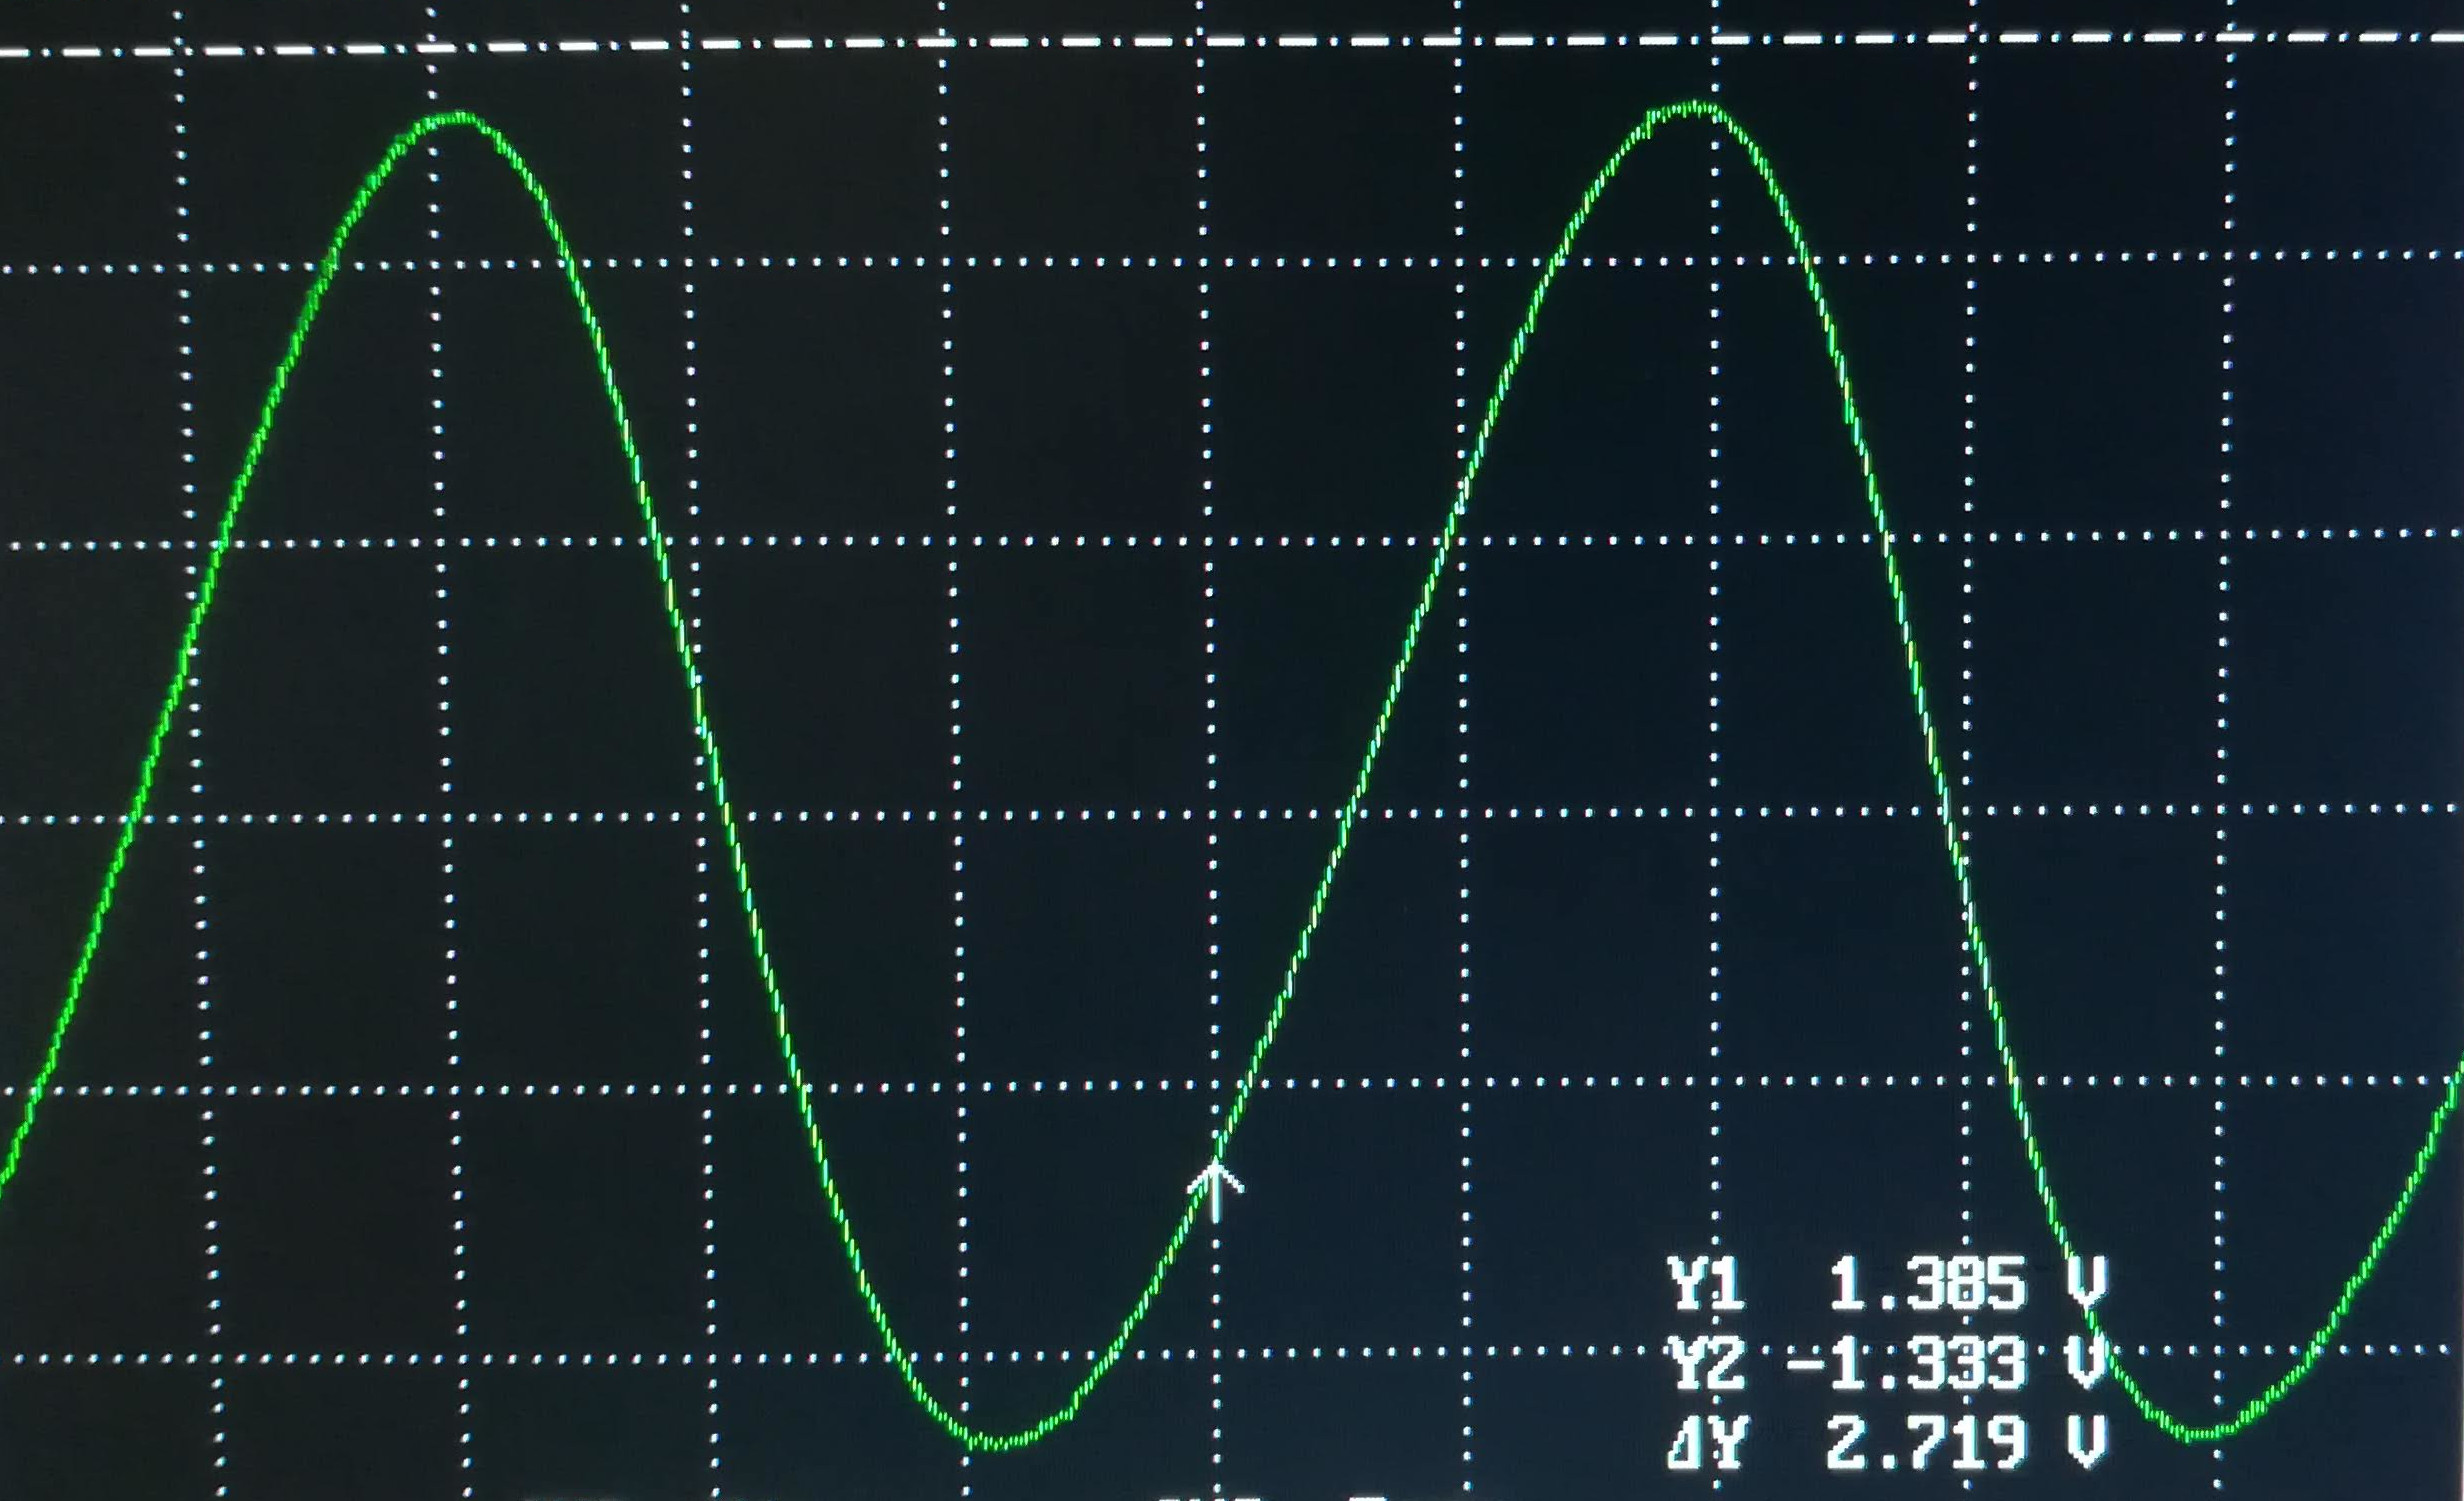
\includegraphics[width=0.6\textwidth]{img/ionicsonic/oscill.jpg}
  \caption{Signal from Langmuir probe: note the distorted sinusoidal wave. Scale: 1 square = $10\si{\micro\second}\times500\si{\milli\volt}$}
  \label{fig:isspeed:oscill}
\end{figure}

Moving the pump-side probe perpendicularly to the grid, the shift of the maximum and minimum of the detected wave has been measured, and thus the speed estimated.

After various tests, searching for a configuration in which the non linear effects (i.e. the distortion of the sinusoidal wave at various position of the probe) can be neglected, the pressure has been set to around $3.26\cdot10^{-3}\si{\milli\bar}$ and the polarization voltage to $36.0\si{\volt}$. The following measurements have been done:
\begin{table}[H]
  \centering
  \begin{tabular}{cccccccc}
    \toprule
    $\Delta x [\si{\milli\metre}]$ & $\Delta t_{min} [\si{\micro\second}]$ & $\Delta t_{max} [\si{\micro\second}]$ \\
    \midrule
    $5.0\pm0.1$ & $2.0\pm0.2$ & $5.0\pm0.2$\\
    $10.0\pm0.1$ & $5.0\pm0.2$ & $7.0\pm0.2$\\
    \bottomrule
  \end{tabular}
  \caption{IonicSonic speed: maximum and minimum shifts}
  \label{tab:isspeed}
\end{table}

By computing the speed $c_s$ as $\frac[f]{\Delta x}{\Delta t}$ in both cases and then taking the average one obtains:

\begin{gather*}
  c_{s,min} \sim 1.3\cdot10^{3} \si{\metre\per\second} \\
  c_{s,max} \sim 2.3\cdot10^{3} \si{\metre\per\second} \\
  c_s \sim 1.8\cdot10^{3} \si{\metre\per\second}
\end{gather*}
In a first approximation,
\begin{equation*}
  c_s = \sqrt{\frac{k_B T_e}{m_i}}
\end{equation*}
where $m_i$ is the Argon-ion mass ($m_i\sim6.63\cdot10^{-26}\si{\kilo\gram}$), which lead to an estimated electron temperature of:
\begin{equation*}
  T_e \sim 1.3\si{\electronvolt}
\end{equation*}

Observe that these estimations are very coarse; the used method, the available apparatus and the non-linearity terms doesn't allow a better result.

When this result are compared to the previous ones, we can see similarity both in the ionic--sonic speed and in the temperature value.

Nevertheless if we consider graph \ref{fig:Te}(d) and \ref{fig:cs}(d) is clear that variation of the pressure in the chamber raise to evident shift in electronic temperature and ionic--sonic speed. The difference in pressure between the latters and the previous data may raise to the gap between the two results. Also variations of the Debye sheath could be origin of experimental data which are different from theoretical ones.

\section{IonicSonic decay}
Keeping the same system conditions, the amplitude of the wave as function of the probe position has been studied. Moving the probe perpendicularly to the grid and recording the amplitude of the wave, the trend in fig. \ref{fig:ionicsonic:expdecay} are found.

\begin{figure}[H]
  \centering
  \resizebox{0.8\textwidth}{!}{\import{img/ionicsonic/}{amplitude.tex}}
  \caption{Peak-peak amplitude of the wave as function of the position. The $0$ in the x axis has been chosen to be about around the middle of the plot.}
  \label{fig:ionicsonic:expdecay}
\end{figure}

From the theory, the amplitude should decay as an exponential. The low range explored doesn't permit a proper exponential fit, thus a first-order approximation around an arbitrary $d_0$ (a zero in the position is not available, therefore an arbitrary offset must be taken in account) has been done:
\begin{equation*}
  Ae^{-\frac[f]{d}{\lambda}} = Ae^{-\frac[f]{(d-d_0+d_0)}{\lambda}} =  \underbrace{Ae^{-\frac[f]{d_0}{\lambda}}}_{a} \left( 1 - \frac{d-d_0}{\lambda}\right)
\end{equation*}

Having chosen in the plot the $x$ axis such that it has the $0$ around the middle of the fit range, can be assumed $x = d-d_0$. From the fit, the typical length is found:
\begin{equation*}
  \lambda = ( 0.030 \pm 0.001 )\si{\metre}
\end{equation*}

This length can be approximated by:
\begin{equation*}
  \lambda = \frac{2c_s}{v_{te}n_0\sigma_0}
\end{equation*}
being $\sigma_0$ the cross section of the collisions of electrons with the neutrals ($\sigma_0\sim2\cdot10^{-20}\si{\metre\squared}$), $c_s$ the previous found ionic-sonic speed and $v_{te}$ the electrons thermal speed ($v_{te}\sim\sqrt{\frac[f]{3k_bT_e}{m_e}}\sim8.4\cdot10^{5}\si{\metre\per\second}$). This lead to an estimation of the neutral particle density $n_0$ of:
\begin{equation*}
  n_0 \sim 7\cdot10^{18} \si{\metre^{-3}}
\end{equation*}

On the other hand, from the perfect-gas law, we can instead compute (assuming a temperature near to the room one, $\sim300\si{\kelvin}$):
\begin{equation*}
  p = nk_BT\quad\rightarrow\quad n = \frac{p}{k_BT} \sim 8\cdot10^{19} \si{\metre^{-3}}
\end{equation*}

The two estimations are clearly incompatible: they differs from an order of magnitude. This can be due to the multiple approximations made to compute $n_0$. First of all the fit: the explored range is too narrow to appreciate the exponential shape, and the trick used make our estimation rougher. Moreover, the multiple approximate values used contribute to a inaccurate estimation of the neutral density.

\section{Conclusions}
With respect to the initial aims:
\begin{itemize}
  \item By studying the vacuum, the average inflow in the chamber and the pumping speed of the pumping system have been estimated.
  \item By studying the V-I characteristics of the tungsten filament the relation between the filament current and its temperature has been found.
  \item The V-I characteristics of the plasma in DC condition has been found and the Paschen curve built: both of them show relevant deviation from the theory.
  \item \todo[inline]{Paschen RF results}
  \item The analysis of plasma parameter throw Langmuir probes showed several dependence of plasma parameter on apparatus settings. In particular, we notice how pressure strongly influence the working conditions of the plasma, while a growth of filament current typically raise to higher values of plasma parameters, i.e. electronic temperature, ionic sonic speed, plasma potential, and plasma density, with an approximatively linear dependence (in same case a kind of saturation in the growth has been seen).
  \item By inducing a sonic wave in the plasma the ionic sonic speed and the wave exponential damping have been estimated.
\end{itemize}


\todo[inline]{Commenti sulla dipendenza di Vf da V. -> File Langmuir/Vf.tex. Non so a cosa vi serva ma nel file c'è il grafico carino.}
\todo[inline]{Dire qualcosa sul fatto che le due stime di $n_0$ differiscono di un'ordine di grandezza}



\end{document}
